\section{卤代酸}

\subsection{$\alpha$-卤代酸}

卤原子受到羰基的影响,反应活性增强,因此易与各种亲核试剂发生反应,生成$\alpha$-取代羧酸。


\subsubsection{酸性}

\begin{center}
    $\ce{RCH2COOH}$ < \small\chemfig{R-CH(-[:90]Cl)-COOH} > \chemfig{R-CH(-[:90]OH)-COOH}
\end{center}


中间的羟基吸电子能力没有 $\ce{-OH}$ 强。这是因为 $\ce{-OH}$ 的氧原子还连着一个 $\ce{H}$ ,削弱了 $\ce{O}$  吸电子的能力。


\subsubsection{亲核取代}

\textbf{合成丙二酸二乙酯的反应} 

\textcolor{red}{要求记忆!}

\begin{center}
    \small
    \schemestart
    \chemfig{CH_2=CH_2} \arrow \chemfig{CH_2(-[:30]COOC_2H_5)-[:-30]COOC_2H_5}
    \schemestop
\end{center}

\begin{figure}[H]
    \centering
    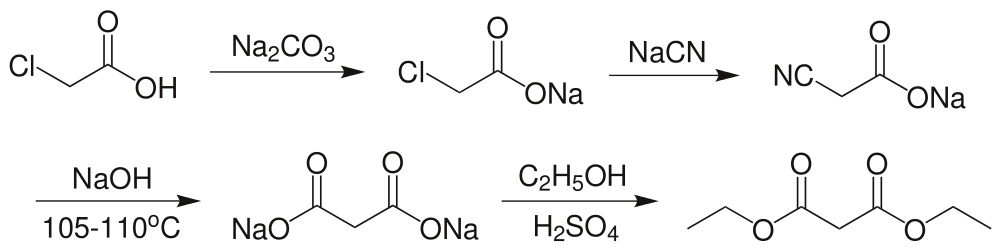
\includegraphics[width=0.8\textwidth]{img/1000px-Diethyl_malonate_synthesis.svg.png}
\end{figure}

\subsection{$\beta$ - 卤代酸}


性质上和$\alpha$卤代酸的性质差不多。外加可以进行消去反应。
